% !TEX TS-program = pdflatex
% !TEX encoding = UTF-8 Unicode
% 
% This is a simple template for a LaTeX document using the "article" class.
% See "book", "report", "letter" for other types of document.
% 
\documentclass[11pt]{article} % use larger type; default would be 10pt
% 
% 
% 
%%% The "real" document content comes below...
\input{header}
% 
\title{Introduction to Math for DS Group Task 2}
\author{IMDS Group 24 \\ Zehao Qian, Mohammad Jamshaid Iqbal, Chloe Mendez}
\begin{document}
\maketitle
% 
% 
% \input{example}
\section{Question 1}
% 
% 
% 
\paragraph{If \( A = \begin{bmatrix}
        1 & 0 & 4 & 1  \\
        0 & 2 & 0 & 2  \\
        6 & 0 & 3 & 11 \\
    \end{bmatrix} \)
    ,
    \( B = \begin{bmatrix}
        7 & -1 & 2 \\
        1 & 1  & 0 \\
        2 & 0  & 1 \\
    \end{bmatrix} \). What is the product AB?}
% 
% 
$$$$
% 
% 
\begin{lstlisting}[style=pystyle]
import numpy as np

# Define the matrices A and B
A = np.array([
    [1, 0, 4, 1],
    [0, 2, 0, 2],
    [6, 0, 3, 11]
])

B = np.array([
    [7, -1, 2],
    [1, 1, 0],
    [2, 0, 1]
])

# Calculate the product of A and B
AB_product = np.dot(A, B)
AB_product    
\end{lstlisting}
% 
% 
% 
% 
\paragraph{\textcolor{red}{Return ValueError: shapes (3,4) and (3,3) not aligned: 4 (dim 1) != 3 (dim 0)}}
% 
% 
\paragraph{\textbf{Analytics:} The product of two matrices AB is undefined if the number of columns in the first matrix A does not match the number of rows in the second matrix B. In this case, matrix A has 4 columns, while matrix B has 3 rows, so their product cannot be computed. Matrix multiplication requires that the number of columns in the first matrix be equal to the number of rows in the second matrix. If there's a third matrix C that should be involved to make the multiplication possible, please provide it, otherwise matrix A and B as given cannot be multiplied.}
% 
% 
% 
% 
% 
% 
% 
% 
% 
% 
% 
% 
% 
% 
\section{Question 2}
\paragraph{What is the dimension of the span of the vectors $(5,7,9,0)$, $(2,5,0,1)$, $(0,0,0,1)$ and $(7,12,9,3)$?}
% 
% 
% 
% 
$$$$
% 
% 
% 
\begin{lstlisting}[style=pystyle]
import numpy as np

# Define the vectors
vectors = np.array([
    [5, 7, 9, 0],
    [2, 5, 0, 1],
    [0, 0, 0, 1],
    [7, 12, 9, 3]
])

# Using numpy to find the rank of the matrix composed of the given vectors
rank_of_matrix = np.linalg.matrix_rank(vectors)
rank_of_matrix
\end{lstlisting}
% 
% 
% 
% 
\paragraph{\textbf{Analytics:} The four vectors $(5,7,9,0)$, $(2,5,0,1)$, $(0,0,0,1)$, and $(7,12,9,3)$ are actually linearly related, because the dimensions of the space they stretch are 3, not 4. This means that of the four vectors, at least one can be linearly represented by the other three. To find a set of linearly independent vectors, we need to remove at least one of the vectors so that the rank of the remaining set of vectors equals the number of vectors. In this example, since any three of these four vectors can form a basis of a stretched space, a linearly independent set of vectors can be obtained by removing any one of them.}
% 
% 
% \subsection{AI Answers}
% \paragraph{Since we used multiple rounds of dialogue to try to correct the answers generated by LLM, it was not aesthetically pleasing to paste into the document due to too much content. That's why we've taken the approach of sharing a history of conversations.}
% \begin{mdframed}[
%         backgroundcolor=white,  % 背景颜色
%         linecolor=black,        % 边框颜色
%         leftmargin=5pt,         % 左边距
%         rightmargin=5pt,        % 右边距
%         linewidth=2pt           % 边框的宽度
%     ]
%     \textbf{ChatGPT's Answer: } \\
%     \href{https://chat.openai.com/share/6e64d98d-8d06-4575-bf97-e6e721612e47}{https://chat.openai.com/share/6e64d98d-8d06-4575-bf97-e6e721612e47} \\
%     \textbf{Bard's Answer: } \\
%     \href{https://g.co/bard/share/983927e7e284}{https://g.co/bard/share/983927e7e284}
% \end{mdframed}
% % 
% % 
% % 
% % 
% \subsection{Analytics:}
% \paragraph{In three-dimensional space, we can calculate the distance from a point to a line using the following formula:}
% \paragraph{Let's say you have a point X with coordinates $(x_0, y_0, z_0)$, and a line defined by two points O$(0,0,0)$ and P$(2,2,1)$. The Projection formula is:}
% % 
% $$ Proj_{L}X = \frac{\vec{X} \cdot \vec{OP}}{\vec{OP} \cdot \vec{OP}} * \vec{OP} $$
% % 
% \paragraph{Then to find the distance, we will use:}

% $$
%     distance = ||\vec{x} - Proj_{L}X||
% $$
% % 
% % $$ d = \frac{|(\mathbf{P} - \mathbf{A}) \cdot \mathbf{n}|}{|\mathbf{AB}|} $$
% \tikzset{every picture/.style={line width=0.75pt}} %set default line width to 0.75pt        

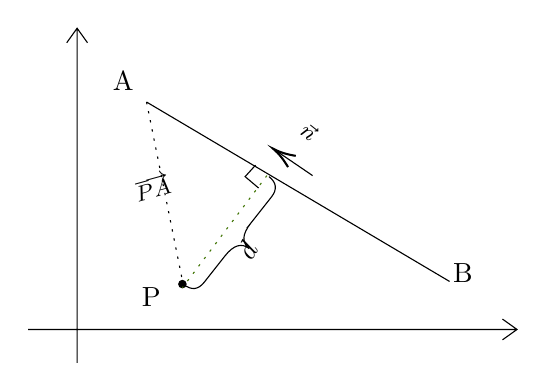
\begin{tikzpicture}[x=0.75pt,y=0.75pt,yscale=-1,xscale=1]
    %uncomment if require: \path (0,210); %set diagram left start at 0, and has height of 210

    %Shape: Axis 2D [id:dp44317292301248945] 
    \draw  (50,159.58) -- (285.5,159.58)(73.55,14.45) -- (73.55,175.7) (278.5,154.58) -- (285.5,159.58) -- (278.5,164.58) (68.55,21.45) -- (73.55,14.45) -- (78.55,21.45)  ;
    %Straight Lines [id:da2979242010824248] 
    \draw    (107,50) -- (253,136.45) ;
    %Shape: Circle [id:dp023999541748674025] 
    \draw  [fill={rgb, 255:red, 0; green, 0; blue, 0 }  ,fill opacity=1 ] (122.5,137.73) .. controls (122.5,136.75) and (123.29,135.95) .. (124.27,135.95) .. controls (125.25,135.95) and (126.05,136.75) .. (126.05,137.73) .. controls (126.05,138.71) and (125.25,139.5) .. (124.27,139.5) .. controls (123.29,139.5) and (122.5,138.71) .. (122.5,137.73) -- cycle ;
    %Straight Lines [id:da4396600304527325] 
    \draw    (187,85.45) -- (169.65,73.63) ;
    \draw [shift={(168,72.5)}, rotate = 34.28] [color={rgb, 255:red, 0; green, 0; blue, 0 }  ][line width=0.75]    (10.93,-3.29) .. controls (6.95,-1.4) and (3.31,-0.3) .. (0,0) .. controls (3.31,0.3) and (6.95,1.4) .. (10.93,3.29)   ;
    %Straight Lines [id:da11083812462923981] 
    \draw  [dash pattern={on 0.84pt off 2.51pt}]  (107,50) -- (124.27,135.95) ;
    %Straight Lines [id:da3033500048537672] 
    \draw [color={rgb, 255:red, 65; green, 117; blue, 5 }  ,draw opacity=1 ] [dash pattern={on 0.84pt off 2.51pt}]  (165,85.45) -- (124.27,139.5) ;
    %Shape: Brace [id:dp9223930624399752] 
    \draw   (125,137.95) .. controls (128.67,140.84) and (131.94,140.46) .. (134.83,136.79) -- (144.8,124.14) .. controls (148.93,118.91) and (152.83,117.73) .. (156.49,120.62) .. controls (152.83,117.73) and (153.06,113.67) .. (157.19,108.43)(155.33,110.79) -- (167.16,95.78) .. controls (170.05,92.11) and (169.66,88.84) .. (166,85.95) ;
    %Straight Lines [id:da5740957717017106] 
    \draw    (159.5,80.45) -- (154.5,85.95) -- (161,91.45) ;

    % Text Node
    \draw (89.5,34) node [anchor=north west][inner sep=0.75pt]   [align=left] {A};
    % Text Node
    \draw (253.5,126.5) node [anchor=north west][inner sep=0.75pt]   [align=left] {B};
    % Text Node
    \draw (103.5,138) node [anchor=north west][inner sep=0.75pt]   [align=left] {P};
    % Text Node
    \draw (184.96,57.48) node [anchor=north west][inner sep=0.75pt]  [font=\footnotesize,rotate=-38.36]  {$\vec{n}$};
    % Text Node
    \draw (147.97,122.08) node [anchor=north west][inner sep=0.75pt]  [rotate=-302.14]  {$d$};
    % Text Node
    \draw (98.59,87.74) node [anchor=north west][inner sep=0.75pt]  [font=\footnotesize,rotate=-344.6]  {$\overrightarrow{PA}$};


\end{tikzpicture}
% % 
% % 
% \subsection{Code for calculation}
% \begin{itemize}
%     \item We calculate the distance from A, B, C, D, E by using Python in a Jupyter Notebook and define a function called \textbf{point\_to\_line\_distance}. The code is below:
% \end{itemize}
% % 
% % 
% % 
% \begin{lstlisting}[style=pystyle]
% import numpy as np

% # Define the coordinates of the two points 
% # that define the line L
% point_O = np.array([0, 0, 0])
% point_P = np.array([2, 2, 1])

% # Define the coordinates of points A, B, C, D, and E
% point_A = np.array([8, 9, 0.9])
% point_B = np.array([4, 4, 2.1])
% point_C = np.array([0.9, 0.99, 0.49])
% point_D = np.array([-2, -2, 1])
% point_E = np.array([0, 2.1, 0])

% # Function to calculate the distance from a point to a line


% def point_to_line_distance(point, line_point_O, line_point_P):
%     line_vector = line_point_P - line_point_O
%     point_vector = point - line_point_O
%     distance = np.linalg.norm(
%         np.cross(line_vector, point_vector)) / np.linalg.norm(line_vector)
%     return distance


% # Calculate and print the distances
% dist_A = point_to_line_distance(point_A, point_O, point_P)
% dist_B = point_to_line_distance(point_B, point_O, point_P)
% dist_C = point_to_line_distance(point_C, point_O, point_P)
% dist_D = point_to_line_distance(point_D, point_O, point_P)
% dist_E = point_to_line_distance(point_E, point_O, point_P)

% print(f"Distance from point A to line L: {dist_A}")
% print(f"Distance from point B to line L: {dist_B}")
% print(f"Distance from point C to line L: {dist_C}")
% print(f"Distance from point D to line L: {dist_D}")
% print(f"Distance from point E to line L: {dist_E}")
% \end{lstlisting}
% \paragraph{The output is: }
% \begin{itemize}
%     \item Distance from point A to line L: 3.2365962917168947
%     \item Distance from point B to line L: 0.09428090415820643
%     \item Distance from point C to line L: 0.06574360974438671
%     \item Distance from point D to line L: 1.885618083164127
%     \item Distance from point E to line L: 1.565247584249853
% \end{itemize}

% \paragraph{\textbf{So the conclusion is: $d(A)>d(D)>d(E)>d(B)>d(C)$}}


% % 
% \begin{figure}[H]
%     \centering
%     \includegraphics[width=0.5\textwidth]{pic/DrawPlot.png}
%     \caption{We draw this picture with Matplotlib in Jupyter Notebook}
% \end{figure}
% % 
% % 
% % 
% \subsection{AI Analytics}
% \paragraph{\textbf{ChatGPT} the use of dot product in the numerator by ChatGPT is wrong for example in
%     ProjLA, the dot product (8,9,0.9).(2,2,1) that ChatGPT is giving us is 26 whereas it should
%     be 34.9. It made the same mistakes for all the Projections of the other points. Due to this
%     mistake, it got the wrong projection which in turn gave the wrong distances from the defined
%     point to the line L. ChatGPT gave the answer A to be the smallest distance and D to be
%     the farthest. The smallest distance actually is C not A, the farthest distance is A not D.
%     Again this shows that due to ChatGPT calculating wrong it gives the wrong answer.}
% \paragraph{\textbf{Bard} is giving a bit weird calculation as it is adding the point’s vector by the points first
%     number. Due to this the dot product, it is giving for each and every point is wrong and in
%     turn the projection it gave was also wrong which resulted in taking out the wrong distances.
%     But surprisingly the answer of the shortest distance it calculated is right which is C whereas
%     the longest distance it calculated it to be D which is wrong.}

% \paragraph{After asking both the chats to reconsider their answer they still were giving the same answer.}


% \begin{itemize}
%     \item \(\mathbf{P} - \mathbf{A}\) represents the vector from point A to point P.
%     \item \(\mathbf{AB}\) represents the vector along the line from point A to point B.
%     \item \(\cdot\) denotes the dot product between vectors.
%     \item \(\mathbf{n}\) is the unit vector along the line AB, which is given by \(\frac{\mathbf{AB}}{|\mathbf{AB}|}\).
% \end{itemize}
% % 
% 
% 
% 
% 
% 
% 
% 
% 
% 
% % 
% % 
% % 
% % 
% % 
% % 
% % 
% % 
% \subsection{AI Answers}
% \begin{mdframed}[
%         backgroundcolor=white,  % 背景颜色
%         linecolor=black,        % 边框颜色
%         leftmargin=5pt,         % 左边距
%         rightmargin=5pt,        % 右边距
%         linewidth=2pt           % 边框的宽度
%     ]
%     \textbf{ChatGPT's Answer: } \\
%     \href{https://chat.openai.com/share/00f22dd3-31f5-4654-95fe-bae6bf2763f1}{https://chat.openai.com/share/00f22dd3-31f5-4654-95fe-bae6bf2763f1} \\
%     \textbf{Bard's Answer: } \\
%     \href{https://g.co/bard/share/aae3031772cb}{https://g.co/bard/share/aae3031772cb}
% \end{mdframed}
% % 
% % 
% % 
% % 
% 
% 
% 
% 
% 
\end{document}
% 